% -------------------------------------------------
% VERSION TRACKER — No modificar este bloque
% Versión:    Tesis Humanizada
% Archivo:    Anexos/AnexoDiagramaFlujo.tex
% Última mod:  2026-05-08T08:45:26
% Git commit:  cc9c766f @ main
% Audiencia:   general
% Verificar antes de editar: bash check_tesis_version.sh overleaf_tesis_humanizado/Anexos/AnexoDiagramaFlujo.tex
% -------------------------------------------------


\section*{Diagrama de flujo del proceso FEFO} \label{flujoFEFO}
\addcontentsline{toc}{section}{Diagrama de flujo del proceso FEFO}

El siguiente diagrama de actividad modela el ciclo de vida completo de un lote bajo la política FEFO (First Expired, First Out — primero en vencer, primero en salir), desde su registro inicial en bodega hasta su despacho final. El flujo incluye dos puntos de decisión críticos: el monitoreo continuo de fechas de vencimiento con alerta a los 15 días, y el algoritmo de selección que itera sobre los lotes activos ordenados por proximidad de vencimiento, descontando del más urgente primero.

\begin{figure}[H]
	\centering
	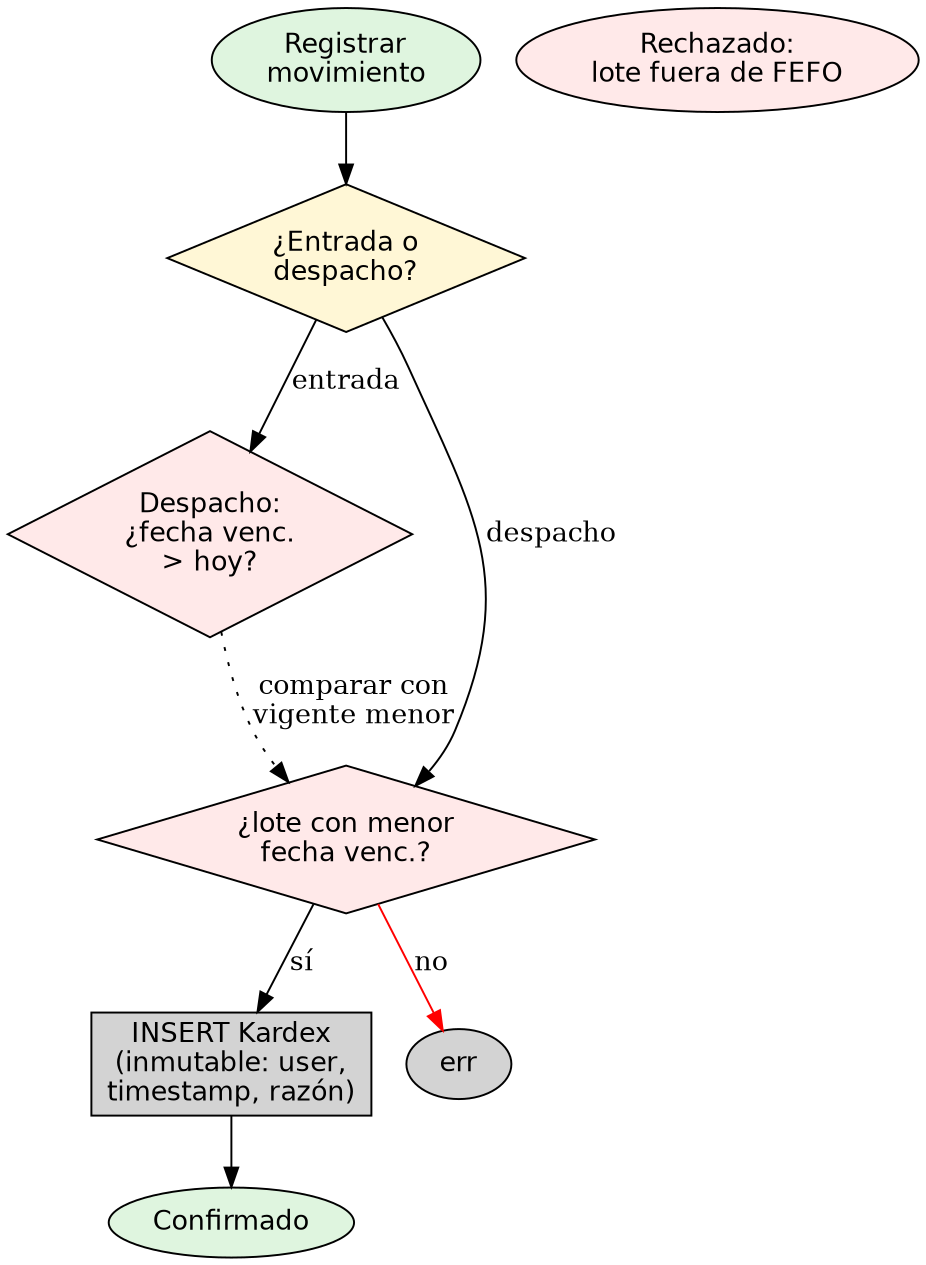
\includegraphics[width=15cm]{Anexos/Imagenes/DiagramaFlujoFEFO.png}
	\caption{Diagrama de actividad del proceso FEFO completo: desde el registro de un lote hasta su despacho, incluyendo monitoreo de vencimientos, alertas críticas y el algoritmo de selección por fecha de expiración.}
	\label{fig:flujoFEFO}
\end{figure}

\subsection*{Explicación del flujo FEFO}

El proceso inicia cuando un operario registra un lote nuevo con su fecha de vencimiento. El sistema almacena el lote con estado \texttt{active} e inicia un monitoreo continuo: si la fecha de vencimiento está a 15 días o menos, se genera una alerta de lote crítico. Cuando un operario solicita un despacho, el sistema verifica que haya stock suficiente del material solicitado. Si la cantidad es suficiente, ejecuta el algoritmo FEFO:

\begin{enumerate}
	\item Ordena todos los lotes activos del material por \texttt{expiration\_date} en orden ascendente.
	\item Toma del lote que vence primero la cantidad necesaria.
	\item Si ese lote no alcanza a cubrir la cantidad solicitada, lo agota completamente (marcándolo como \texttt{consumed}) y continúa con el siguiente lote en orden FEFO.
	\item Por cada lote afectado, registra un movimiento tipo \texttt{salida} en el Kardex inmutable, con el motivo especificado por el operario (producción, venta, desperdicio o ajuste).
	\item Todo el proceso ocurre dentro de una transacción atómica (\texttt{DB::transaction}) que garantiza que, si ocurre algún error, no se modifique ningún lote.
\end{enumerate}

Si el stock total del material es insuficiente para cubrir la cantidad solicitada, el sistema rechaza la operación con un mensaje que indica la cantidad disponible.
